\documentclass[]{article}
\usepackage{lmodern}
\usepackage{amssymb,amsmath}
\usepackage{ifxetex,ifluatex}
\usepackage{fixltx2e} % provides \textsubscript
\ifnum 0\ifxetex 1\fi\ifluatex 1\fi=0 % if pdftex
  \usepackage[T1]{fontenc}
  \usepackage[utf8]{inputenc}
\else % if luatex or xelatex
  \ifxetex
    \usepackage{mathspec}
  \else
    \usepackage{fontspec}
  \fi
  \defaultfontfeatures{Ligatures=TeX,Scale=MatchLowercase}
\fi
% use upquote if available, for straight quotes in verbatim environments
\IfFileExists{upquote.sty}{\usepackage{upquote}}{}
% use microtype if available
\IfFileExists{microtype.sty}{%
\usepackage{microtype}
\UseMicrotypeSet[protrusion]{basicmath} % disable protrusion for tt fonts
}{}
\usepackage[margin=1in]{geometry}
\usepackage{hyperref}
\hypersetup{unicode=true,
            pdftitle={MSc. Research Methods - Statistikteil Lösungen 2018},
            pdfauthor={Gian-Andrea Egeler},
            pdfborder={0 0 0},
            breaklinks=true}
\urlstyle{same}  % don't use monospace font for urls
\usepackage{color}
\usepackage{fancyvrb}
\newcommand{\VerbBar}{|}
\newcommand{\VERB}{\Verb[commandchars=\\\{\}]}
\DefineVerbatimEnvironment{Highlighting}{Verbatim}{commandchars=\\\{\}}
% Add ',fontsize=\small' for more characters per line
\usepackage{framed}
\definecolor{shadecolor}{RGB}{248,248,248}
\newenvironment{Shaded}{\begin{snugshade}}{\end{snugshade}}
\newcommand{\KeywordTok}[1]{\textcolor[rgb]{0.13,0.29,0.53}{\textbf{#1}}}
\newcommand{\DataTypeTok}[1]{\textcolor[rgb]{0.13,0.29,0.53}{#1}}
\newcommand{\DecValTok}[1]{\textcolor[rgb]{0.00,0.00,0.81}{#1}}
\newcommand{\BaseNTok}[1]{\textcolor[rgb]{0.00,0.00,0.81}{#1}}
\newcommand{\FloatTok}[1]{\textcolor[rgb]{0.00,0.00,0.81}{#1}}
\newcommand{\ConstantTok}[1]{\textcolor[rgb]{0.00,0.00,0.00}{#1}}
\newcommand{\CharTok}[1]{\textcolor[rgb]{0.31,0.60,0.02}{#1}}
\newcommand{\SpecialCharTok}[1]{\textcolor[rgb]{0.00,0.00,0.00}{#1}}
\newcommand{\StringTok}[1]{\textcolor[rgb]{0.31,0.60,0.02}{#1}}
\newcommand{\VerbatimStringTok}[1]{\textcolor[rgb]{0.31,0.60,0.02}{#1}}
\newcommand{\SpecialStringTok}[1]{\textcolor[rgb]{0.31,0.60,0.02}{#1}}
\newcommand{\ImportTok}[1]{#1}
\newcommand{\CommentTok}[1]{\textcolor[rgb]{0.56,0.35,0.01}{\textit{#1}}}
\newcommand{\DocumentationTok}[1]{\textcolor[rgb]{0.56,0.35,0.01}{\textbf{\textit{#1}}}}
\newcommand{\AnnotationTok}[1]{\textcolor[rgb]{0.56,0.35,0.01}{\textbf{\textit{#1}}}}
\newcommand{\CommentVarTok}[1]{\textcolor[rgb]{0.56,0.35,0.01}{\textbf{\textit{#1}}}}
\newcommand{\OtherTok}[1]{\textcolor[rgb]{0.56,0.35,0.01}{#1}}
\newcommand{\FunctionTok}[1]{\textcolor[rgb]{0.00,0.00,0.00}{#1}}
\newcommand{\VariableTok}[1]{\textcolor[rgb]{0.00,0.00,0.00}{#1}}
\newcommand{\ControlFlowTok}[1]{\textcolor[rgb]{0.13,0.29,0.53}{\textbf{#1}}}
\newcommand{\OperatorTok}[1]{\textcolor[rgb]{0.81,0.36,0.00}{\textbf{#1}}}
\newcommand{\BuiltInTok}[1]{#1}
\newcommand{\ExtensionTok}[1]{#1}
\newcommand{\PreprocessorTok}[1]{\textcolor[rgb]{0.56,0.35,0.01}{\textit{#1}}}
\newcommand{\AttributeTok}[1]{\textcolor[rgb]{0.77,0.63,0.00}{#1}}
\newcommand{\RegionMarkerTok}[1]{#1}
\newcommand{\InformationTok}[1]{\textcolor[rgb]{0.56,0.35,0.01}{\textbf{\textit{#1}}}}
\newcommand{\WarningTok}[1]{\textcolor[rgb]{0.56,0.35,0.01}{\textbf{\textit{#1}}}}
\newcommand{\AlertTok}[1]{\textcolor[rgb]{0.94,0.16,0.16}{#1}}
\newcommand{\ErrorTok}[1]{\textcolor[rgb]{0.64,0.00,0.00}{\textbf{#1}}}
\newcommand{\NormalTok}[1]{#1}
\usepackage{graphicx,grffile}
\makeatletter
\def\maxwidth{\ifdim\Gin@nat@width>\linewidth\linewidth\else\Gin@nat@width\fi}
\def\maxheight{\ifdim\Gin@nat@height>\textheight\textheight\else\Gin@nat@height\fi}
\makeatother
% Scale images if necessary, so that they will not overflow the page
% margins by default, and it is still possible to overwrite the defaults
% using explicit options in \includegraphics[width, height, ...]{}
\setkeys{Gin}{width=\maxwidth,height=\maxheight,keepaspectratio}
\IfFileExists{parskip.sty}{%
\usepackage{parskip}
}{% else
\setlength{\parindent}{0pt}
\setlength{\parskip}{6pt plus 2pt minus 1pt}
}
\setlength{\emergencystretch}{3em}  % prevent overfull lines
\providecommand{\tightlist}{%
  \setlength{\itemsep}{0pt}\setlength{\parskip}{0pt}}
\setcounter{secnumdepth}{0}
% Redefines (sub)paragraphs to behave more like sections
\ifx\paragraph\undefined\else
\let\oldparagraph\paragraph
\renewcommand{\paragraph}[1]{\oldparagraph{#1}\mbox{}}
\fi
\ifx\subparagraph\undefined\else
\let\oldsubparagraph\subparagraph
\renewcommand{\subparagraph}[1]{\oldsubparagraph{#1}\mbox{}}
\fi

%%% Use protect on footnotes to avoid problems with footnotes in titles
\let\rmarkdownfootnote\footnote%
\def\footnote{\protect\rmarkdownfootnote}

%%% Change title format to be more compact
\usepackage{titling}

% Create subtitle command for use in maketitle
\newcommand{\subtitle}[1]{
  \posttitle{
    \begin{center}\large#1\end{center}
    }
}

\setlength{\droptitle}{-2em}

  \title{MSc. Research Methods - Statistikteil Lösungen 2018}
    \pretitle{\vspace{\droptitle}\centering\huge}
  \posttitle{\par}
    \author{Gian-Andrea Egeler}
    \preauthor{\centering\large\emph}
  \postauthor{\par}
      \predate{\centering\large\emph}
  \postdate{\par}
    \date{January 2019}


\begin{document}
\maketitle

\subsubsection{Musterlösung Aufgabe 2.3S: ANOVA mit
Interaktion}\label{musterlosung-aufgabe-2.3s-anova-mit-interaktion}

\begin{Shaded}
\begin{Highlighting}[]
\CommentTok{# klone den originaler Datensatz}
\NormalTok{df <-}\StringTok{ }\NormalTok{nova }

\CommentTok{# fasst die vier Inhalte der Gerichte zu drei Inhalten zusammen.}
\NormalTok{ df}\OperatorTok{$}\NormalTok{label_content[}\KeywordTok{grep}\NormalTok{(}\StringTok{"Pflanzlich+"}\NormalTok{,df}\OperatorTok{$}\NormalTok{label_content)] <-}\StringTok{ "Vegetarisch"}
 
\CommentTok{# gruppiert Daten gemäss Bedingungen, Menü-Inhalt und Wochen}
\NormalTok{df_ <-}\StringTok{ }\NormalTok{df }\OperatorTok
\StringTok{    }\KeywordTok{group_by}\NormalTok{(condit, label_content, week) }\OperatorTok
\StringTok{    }\KeywordTok{summarise}\NormalTok{(}\DataTypeTok{tot_sold =} \KeywordTok{n}\NormalTok{()) }\OperatorTok
\StringTok{    }\KeywordTok{drop_na}\NormalTok{() }\CommentTok{# lasst die unbekannten Menü-Inhalte weg}


\CommentTok{# überprüft Voraussetzungen für eine ANOVA}
\CommentTok{# Boxplots zeigt klare Varianzheterogenität}
\KeywordTok{ggplot}\NormalTok{(df_, }\KeywordTok{aes}\NormalTok{(}\DataTypeTok{x =} \KeywordTok{interaction}\NormalTok{(label_content, condit), }\DataTypeTok{y =}\NormalTok{ tot_sold)) }\OperatorTok{+}
\StringTok{  }\KeywordTok{geom_boxplot}\NormalTok{(}\DataTypeTok{fill=}\StringTok{"white"}\NormalTok{, }\DataTypeTok{size =} \DecValTok{1}\NormalTok{) }\OperatorTok{+}\StringTok{ }
\StringTok{  }\KeywordTok{labs}\NormalTok{(}\DataTypeTok{x =} \StringTok{"}\CharTok{\textbackslash{}n}\StringTok{Menü-Inhalt"}\NormalTok{, }\DataTypeTok{y =} \StringTok{"Anzahl verkaufte Gerichte pro Woche}\CharTok{\textbackslash{}n}\StringTok{"}\NormalTok{) }\OperatorTok{+}
\StringTok{  }\NormalTok{mytheme}
\end{Highlighting}
\end{Shaded}

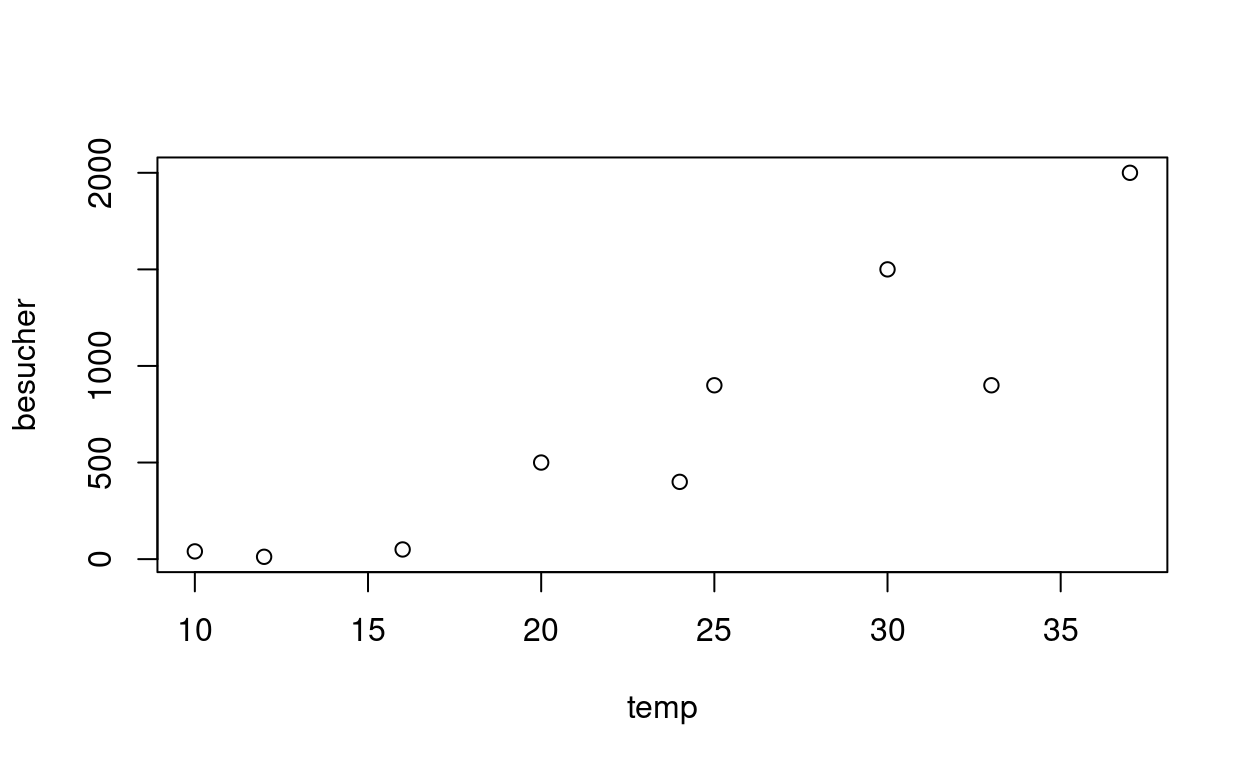
\includegraphics{Musterloesung_Statistik_2.3S_files/figure-latex/unnamed-chunk-2-1.pdf}

\begin{Shaded}
\begin{Highlighting}[]
\CommentTok{# definiert das Modell mit Interaktion}
\NormalTok{model1 <-}\StringTok{ }\KeywordTok{aov}\NormalTok{(tot_sold }\OperatorTok{~}\StringTok{ }\NormalTok{label_content }\OperatorTok{*}\StringTok{ }\NormalTok{condit, }\DataTypeTok{data =}\NormalTok{ df_)}

\KeywordTok{summary.lm}\NormalTok{(model1)}
\end{Highlighting}
\end{Shaded}

\begin{verbatim}
## 
## Call:
## aov(formula = tot_sold ~ label_content * condit, data = df_)
## 
## Residuals:
##     Min      1Q  Median      3Q     Max 
## -6.0000 -4.0000 -0.1667  1.9167  9.3333 
## 
## Coefficients:
##                                             Estimate Std. Error t value
## (Intercept)                                   27.333      3.127   8.741
## label_contentFleisch                          80.333      4.422  18.166
## label_contentVegetarisch                      24.667      4.422   5.578
## conditIntervention                            -3.333      4.422  -0.754
## label_contentFleisch:conditIntervention      -24.000      6.254  -3.838
## label_contentVegetarisch:conditIntervention   28.333      6.254   4.531
##                                             Pr(>|t|)    
## (Intercept)                                 1.50e-06 ***
## label_contentFleisch                        4.27e-10 ***
## label_contentVegetarisch                    0.000120 ***
## conditIntervention                          0.465516    
## label_contentFleisch:conditIntervention     0.002363 ** 
## label_contentVegetarisch:conditIntervention 0.000689 ***
## ---
## Signif. codes:  0 '***' 0.001 '**' 0.01 '*' 0.05 '.' 0.1 ' ' 1
## 
## Residual standard error: 5.416 on 12 degrees of freedom
## Multiple R-squared:  0.9787, Adjusted R-squared:  0.9698 
## F-statistic: 110.3 on 5 and 12 DF,  p-value: 1.334e-09
\end{verbatim}

\begin{Shaded}
\begin{Highlighting}[]
\KeywordTok{autoplot}\NormalTok{(model1) }\OperatorTok{+}\StringTok{ }\NormalTok{mytheme  }\CommentTok{# Inspektion der Modellvoraussetzung: ist ok}
\end{Highlighting}
\end{Shaded}

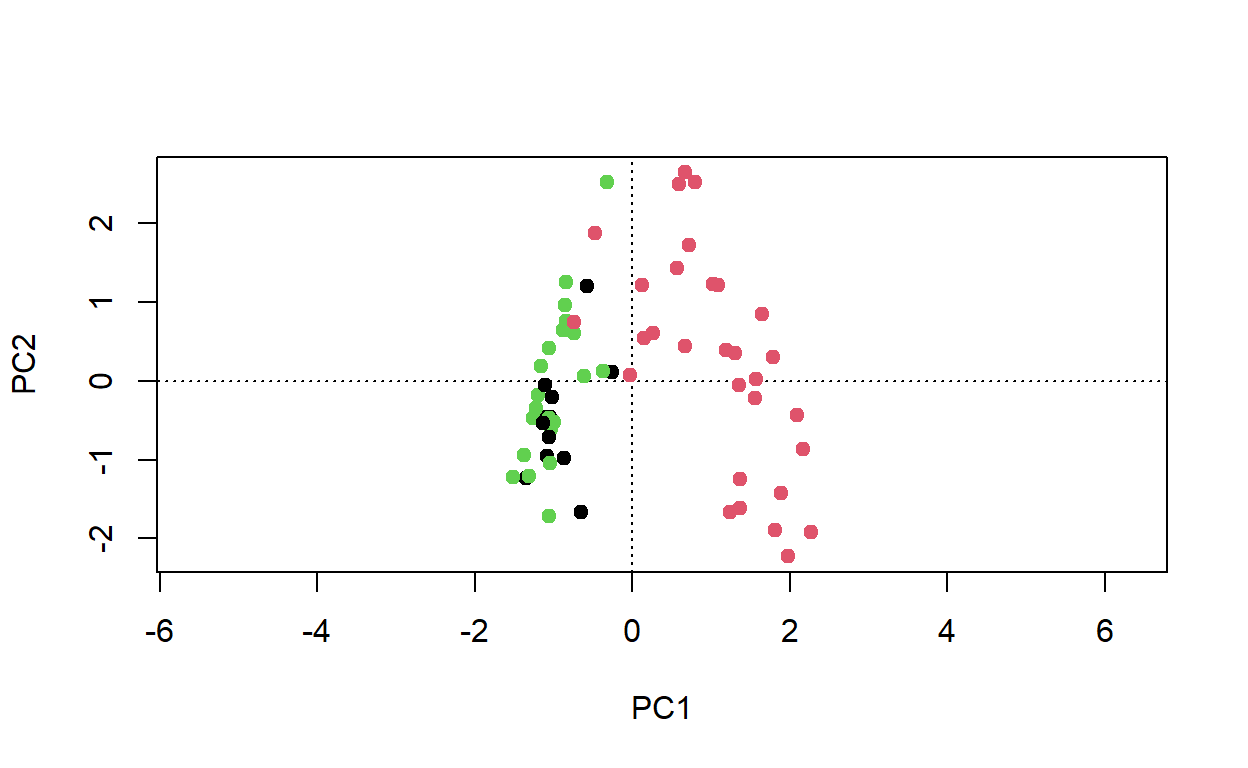
\includegraphics{Musterloesung_Statistik_2.3S_files/figure-latex/unnamed-chunk-2-2.pdf}

Fazit: Die Inspektion des Modells zeigt keine schwerwiegenden
Verletzungen der Modellvoraussetzung. Nächster Schritt post-hoc-Tests
nach Tukey.

\begin{Shaded}
\begin{Highlighting}[]
\CommentTok{# post-hoc-Tests nach Tukey}

\KeywordTok{TukeyHSD}\NormalTok{(model1)}
\end{Highlighting}
\end{Shaded}

\begin{verbatim}
##   Tukey multiple comparisons of means
##     95% family-wise confidence level
## 
## Fit: aov(formula = tot_sold ~ label_content * condit, data = df_)
## 
## $label_content
##                          diff       lwr       upr   p adj
## Fleisch-Buffet       68.33333  59.99107  76.67559 0.0e+00
## Vegetarisch-Buffet   38.83333  30.49107  47.17559 1.0e-07
## Vegetarisch-Fleisch -29.50000 -37.84226 -21.15774 1.9e-06
## 
## $condit
##                         diff       lwr      upr     p adj
## Intervention-Basis -1.888889 -7.451701 3.673923 0.4736291
## 
## $`label_content:condit`
##                                                     diff       lwr
## Fleisch:Basis-Buffet:Basis                     80.333333  65.47963
## Vegetarisch:Basis-Buffet:Basis                 24.666667   9.81296
## Buffet:Intervention-Buffet:Basis               -3.333333 -18.18704
## Fleisch:Intervention-Buffet:Basis              53.000000  38.14629
## Vegetarisch:Intervention-Buffet:Basis          49.666667  34.81296
## Vegetarisch:Basis-Fleisch:Basis               -55.666667 -70.52037
## Buffet:Intervention-Fleisch:Basis             -83.666667 -98.52037
## Fleisch:Intervention-Fleisch:Basis            -27.333333 -42.18704
## Vegetarisch:Intervention-Fleisch:Basis        -30.666667 -45.52037
## Buffet:Intervention-Vegetarisch:Basis         -28.000000 -42.85371
## Fleisch:Intervention-Vegetarisch:Basis         28.333333  13.47963
## Vegetarisch:Intervention-Vegetarisch:Basis     25.000000  10.14629
## Fleisch:Intervention-Buffet:Intervention       56.333333  41.47963
## Vegetarisch:Intervention-Buffet:Intervention   53.000000  38.14629
## Vegetarisch:Intervention-Fleisch:Intervention  -3.333333 -18.18704
##                                                     upr     p adj
## Fleisch:Basis-Buffet:Basis                     95.18704 0.0000000
## Vegetarisch:Basis-Buffet:Basis                 39.52037 0.0012966
## Buffet:Intervention-Buffet:Basis               11.52037 0.9704018
## Fleisch:Intervention-Buffet:Basis              67.85371 0.0000006
## Vegetarisch:Intervention-Buffet:Basis          64.52037 0.0000012
## Vegetarisch:Basis-Fleisch:Basis               -40.81296 0.0000003
## Buffet:Intervention-Fleisch:Basis             -68.81296 0.0000000
## Fleisch:Intervention-Fleisch:Basis            -12.47963 0.0005207
## Vegetarisch:Intervention-Fleisch:Basis        -15.81296 0.0001771
## Buffet:Intervention-Vegetarisch:Basis         -13.14629 0.0004174
## Fleisch:Intervention-Vegetarisch:Basis         43.18704 0.0003741
## Vegetarisch:Intervention-Vegetarisch:Basis     39.85371 0.0011541
## Fleisch:Intervention-Buffet:Intervention       71.18704 0.0000003
## Vegetarisch:Intervention-Buffet:Intervention   67.85371 0.0000006
## Vegetarisch:Intervention-Fleisch:Intervention  11.52037 0.9704018
\end{verbatim}

\paragraph{Methoden}\label{methoden}

Ziel war es, die Unterschiede in den Verkaufszahlen pro Menü-Inhalt und
pro Bedingung aufzuzeigen. Da die Kriteriumsvariable (Verkaufszahlen)
metrisch und die beiden Prädiktorvariablen kategorial sind, wurde eine
zweifaktorielle ANOVA mit Interaktion gerechnet. Die visuelle Inspektion
des Models zeigte keine schwerwiegenden Verletzungen der
Voraussetzungen. Um die Einzelvergleiche zu sehen, wurde einen
post-hoc-Test nach Tukey durchgeführt.

\paragraph{Ergebnisse}\label{ergebnisse}

Die Menü-Inhalte (Fleisch, Vegetarisch und Buffet) zwischen den
Bedingungen Basis oder Interventionswochen unterscheiden sich in den
Verkaufszahlen signifikant (\emph{F}(5, 12) = 110.252, \emph{p}
\textless{} .001). Anschliessend durchgeführte post-hoc-Tests (Tukey)
zeigen vor allem zwei interessante Ergbenisse: 1) in den
Interventionswochen wurden signifikant weniger Fleischgerichte gekauft
als in den Basiswochen 2) in den Interventionswochen wurden signifikant
mehr vegetarische Gerichte verkauft (siehe Figure 1 oder Figure 2).

\begin{figure}
\centering
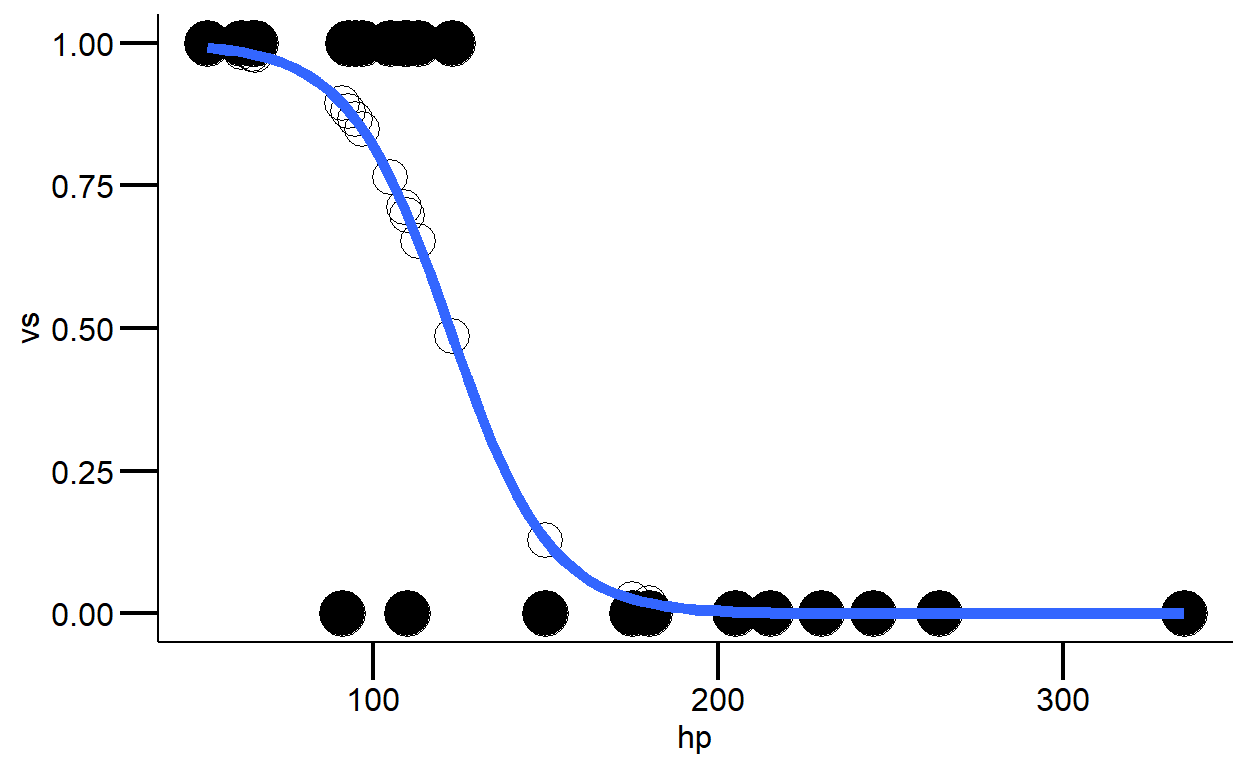
\includegraphics{Musterloesung_Statistik_2.3S_files/figure-latex/unnamed-chunk-4-1.pdf}
\caption{Box-Whisker-Plots der wöchentlichen Verkaufszahlen pro
Menü-Inhalte. Kleinbuchstaben bezeichnen homogene Gruppen auf \emph{p}
\textless{} .05 nach Tukeys post-hoc-Test.}
\end{figure}

\begin{figure}
\centering
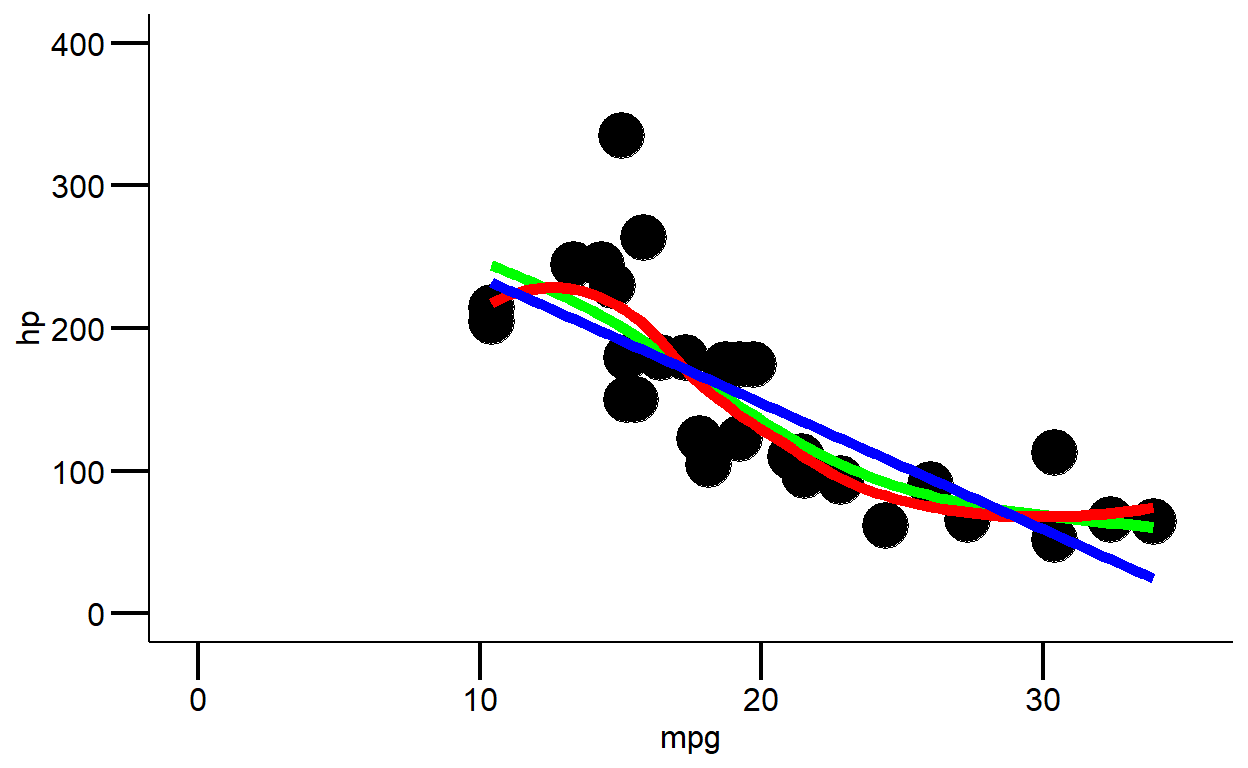
\includegraphics{Musterloesung_Statistik_2.3S_files/figure-latex/unnamed-chunk-5-1.pdf}
\caption{Wöchentliche Verkaufszahlen aggregiert für die drei
Menü-Inhalte.}
\end{figure}


\end{document}
